\documentclass{article}
\usepackage{fullpage}
\usepackage{graphicx}

\def\file#1{\texttt{#1}}
\def\bench#1{\texttt{#1}}
\def\code#1{\texttt{#1}}

\usepackage{caption}
\author{Aur\`ele Barri\`ere \& Benjamin Fasquelle}
\title{Practical Evaluation}
\date{March 24, 2017}

\begin{document}
\maketitle

Except for question 1.1 (on 5 nodes), these experiments were done on 15 nodes.

It would have been better to have several measures for each experiments. With our experiments, we cannot deduce that some strategy will always be better than another one. However, it can show that there are some cases in which some strategy can be better.

\section*{Question 1.1}
To evaluate the usefulness of speculation in a stressed environment, we run several jobs with the same configuration and the same data, the only change being the activation of the speculative execution.

In each job, we are going to stress one of the 5 nodes. In this purpose, we used the script to stress the disk on only one node.

We used the benchmark \bench{sort} with a block size of 128MB, a replication factor of 3 and 8 map/reduce slots.

In the first two runs, we disable the speculation (speculative execution in \file{mapred-site.xml}).
In the next two runs, we enable the speculation.

%to be continued

We used a data set of 20GB, with replication factor 3.

Some results are presented in the Table 1.

\begin{center}
\captionof{table}{Measurement}
\begin{tabular}{|c|c|c|}
\hline
\ & Without speculation & With speculation \\
\hline
Execution time & 5mins, 55sec & 6mins, 58sec \\
\hline
Number of speculatives copies & 0 & 4 \\
\hline
Average Map run time & 3sec & 5sec \\
\hline
Maximum Map run time & 5sec & 11sec \\
\hline
Average Reduce run time & 1mins, 48sec & 2mins, 4sec \\
\hline
Maximum Reduce run time & 2mins, 18sec & 2mins, 40sec \\
\hline
\end{tabular}
\end{center}



Speculative tasks have lower priority, thus we can see on Figure (\ref{spec_prio}) that they are executed at the end (tasks in red).

\begin{figure}%[h!]
  \centering
  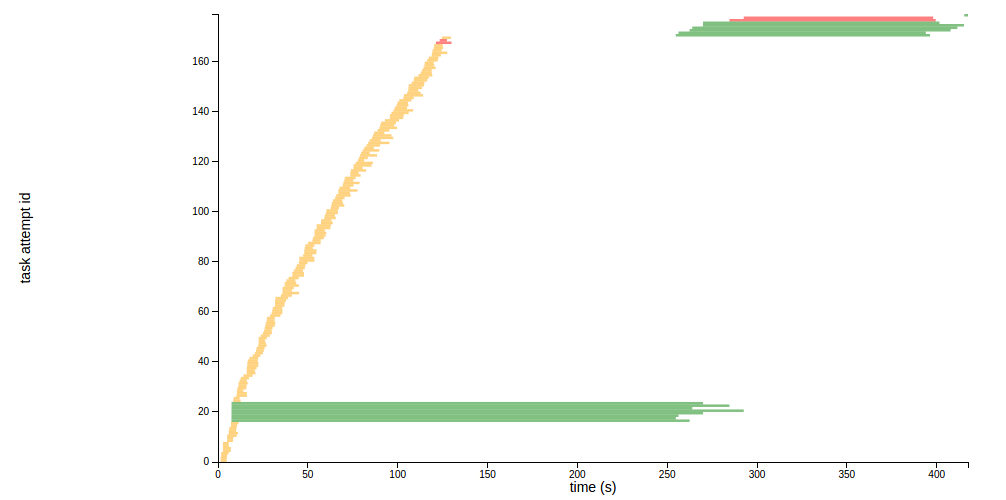
\includegraphics[width=0.6\textwidth]{spec.png}
  \caption{Executions of the tasks with speculation}
  \label{spec_prio}
\end{figure}


It explains why speculative execution is not helpful in this case. Indeed, it should reduce the average and maximum time of the nodes. However, we can see here that speculative tasks are launched int the end and fail. Thus, they are not useful because they do not end sooner than stragglers. They even consume resources that could be used by other nodes to terminate faster.

Thus, it shows that speculative execution is not always a better strategy to reduce execution time.

\section*{Question 1.2}

We used a data set of 20GB and run sort benchmark using block size at 128MB and the replication factor at 3.

We execute runs with different expiry interval (30seconds and 1 minute), and stop the tasktracker daemon on one node (one time before the completion of the map tasks, another after this completion).

The next tables show the execution times and the number of killed tasks respectively.

\begin{center}
\captionof{table}{Execution times} 
\begin{tabular}{|c|c|c|}
\hline
\ & expiry interval: 30 seconds & expiry interval: 1 minute \\
\hline
Before completion map & 8mins, 58sec & 14mins, 3sec \\
\hline
After completion map & 14mins, 41sec & 12mins, 27sec\\
\hline
\end{tabular}
\end{center}

\begin{center}
\captionof{table}{Number of killed tasks} 
\begin{tabular}{|c|c|c|}
\hline
\ & expiry interval: 30 seconds & expiry interval: 1 minute \\
\hline
Before completion map & 4 & 11 \\
\hline
After completion map & 21 & 13 \\
\hline
\end{tabular}
\end{center}


\begin{figure}%[h!]
  \centering
  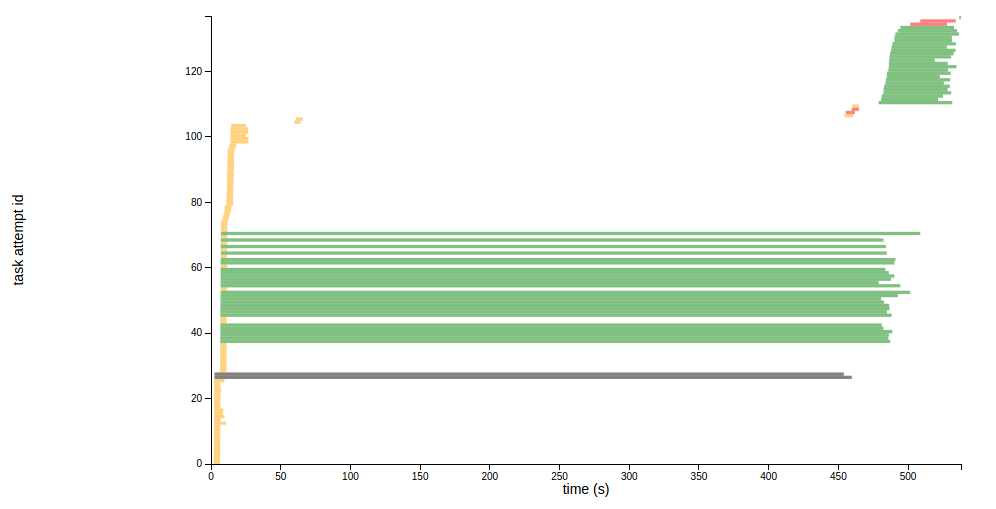
\includegraphics[width=0.4\textwidth]{expiry30before.png}
  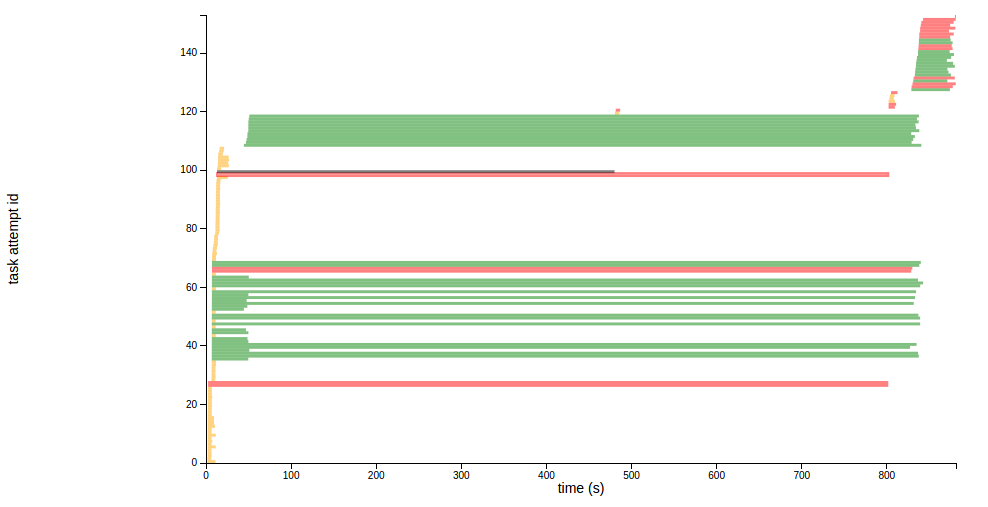
\includegraphics[width=0.4\textwidth]{expiry30after.png}
  \caption{Left: Tasktracker daemon stop before (left) and after (right) the completion of the map tasks (30sec)}
  \label{kill}
\end{figure}


First, we can see that increasing the expiry time can make the execution time longer. Indeed, for every failed node, the master node will detect it less qickly, and then the backup tasks will be launched much later. However, in our experiments, it does not always increase the execution time.

We can also see that there are more killed tasks when we kill the tasktracker after the completion of the map tasks. Indeed, when a node is killed, we looses both the map results that he had and the work he had done on the reduce phase. When we killed the tasktracker after the end of the map tasks, we actually saw the percentage of map completion go backward, because some map tasks had to be done again.

\section*{Question 2.1}


We used a data set of 10GB and run wordcount and sort benchmarks using
different values (0.05, 0.5, and 1) of slowstart.
It means that the reduce phase will only start of some percentage of the map phase is done (5\%, 50\% or 100\%).

The next table shows the execution times.

\begin{center}
\captionof{table}{Execution times} 
\begin{tabular}{|c|c|c|}
\hline
\ & Sort & Wordcount \\
\hline
0.05 & 1mins, 2sec & 6mins, 55sec \\
\hline
0.5 & 1mins, 19sec & 6mins, 36sec \\
\hline
1 & 1mins, 7sec & 6mins, 52sec \\
\hline
\end{tabular}
\end{center}

For the sort benchmarks, we can see that the time taken by Map tasks is the same for all the values (3sec in average, 7 at worst).
However, the time taken by Shuffle decreases when the value increases: in average, it is 15sec for 0.05 (18 at worst), 12sec for 0.5 (17 at worst) and 11sec for 1 (14 at worst). For the time taken by Reduce tasks, it's more quickly with the slowstart at 0.5: it is 7sec in average (11 at worst), against 11sec for 0.05 (17 at worst) and 10sec for 1 (14 at worst).
%We can observe that if we want to reduce the global execution time, we can increase the value, that is reduce the Shuffle time, but the Reduce time is lower for the value at 0.5.

For the Wordcount benchmarks, we can see the same thing for the Map time and the Shuffle time, but for the Reduce time, it decreases when the value of slowstart increases: on average, it is 4 minutes and 26sec for 0.05 (4mins, 45 seconds at worst), 3 minutes and 46sec for 0.05 (4 minutes, 15 seconds at worst) and 3 minutes and 40sec for 1 (3 minutes, 59 seconds at worst).


These executions times highlight the fact that a big slowstart can reduce the execution time as well as increase it, depending on the situation.
With a quick start of the reduce nodes, you can sometimes have a better parallelization and start doing useful computations with your reduce nodes early.
With a slower start, for applications that require the end of the map phase before starting the reduce phase (wordcount for instance), you won't benefit from starting the reduce phase early, and it will even use some resources that could have been used for the map phase.

It explains why there is no clear tendency in our experiments. Sometimes a slower start is better, sometimes a quicker one is better. It also depends on the application. Wordcount has a less significant reduce phase than sort, and thus the difference in execution time is less visible.



\begin{figure}%[h!]
  \centering
  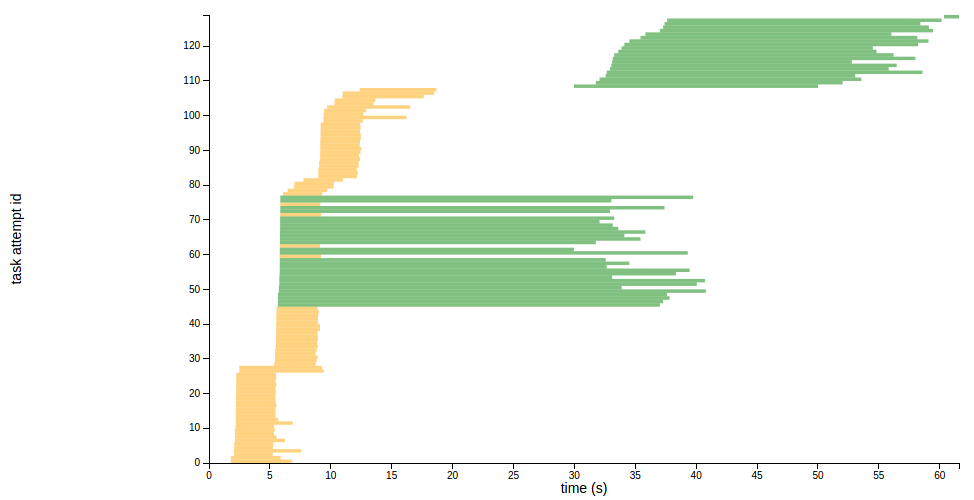
\includegraphics[width=0.4\textwidth]{sort005.png}
  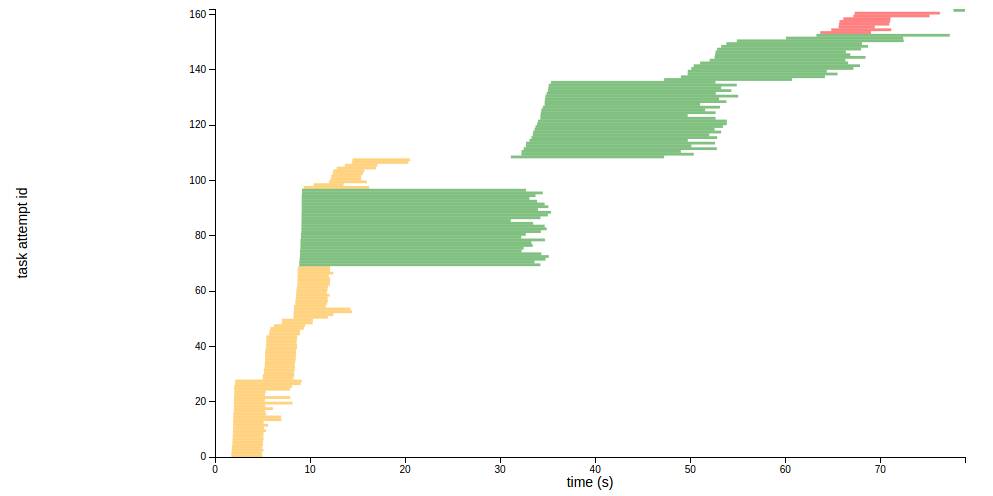
\includegraphics[width=0.4\textwidth]{sort05.png}
  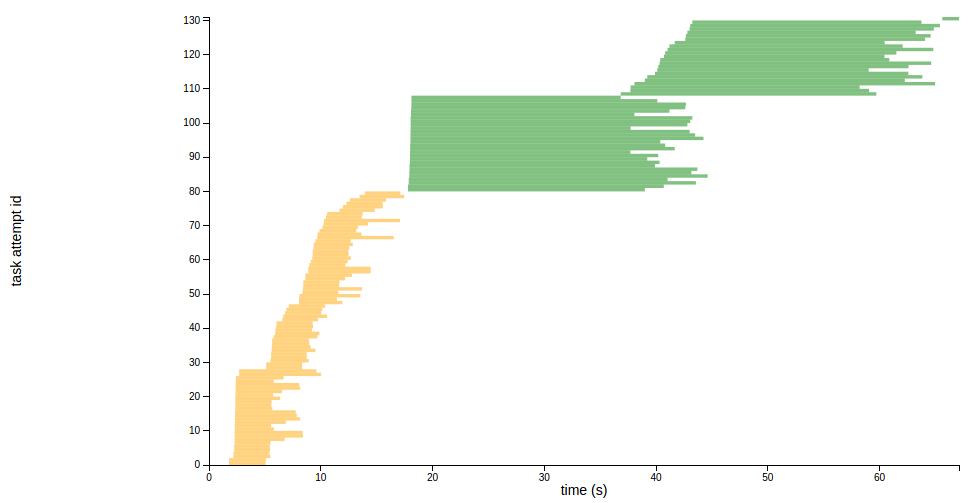
\includegraphics[width=0.4\textwidth]{sort1.png}
  \caption{Sort with value at 0.05 (left), 0.5 (right) and 1 (below)}
  \label{values}
\end{figure}

We can see on Figure (\ref{values}) that the start of the Reduce tasks depends on the value of slowstart, as expected.



\section*{Question 3.1}


We run 6 sort applications on different sizes (3*2GB, 2*4GB 1*10GB) under FIFO scheduler, Fair scheduler (preemption disabled), and Fair scheduler
(preemption enabled) (we used Fair scheduler within the pool).

Jobs were launched with a decreasing input size order and 10 second interval between two
jobs.

%See the execution time, data locality and the waiting time of the applications. what can
%you observe?

The next table shows the execution times.

\begin{center}
\captionof{table}{Execution times} 
\begin{tabular}{|c|c|c|c|}
\hline
\ & FIFO & Fair & Fair with preemption \\
\hline
2GB & 36sec & 31sec & 31sec \\
\hline
2GB & 36sec & 30sec & 30sec \\
\hline
2GB & 38sec & 28sec & 31sec \\
\hline
4GB & 48sec & 46sec & 36sec \\
\hline
4GB & 53sec & 52sec & 37sec \\
\hline
10GB & 1 minute, 17sec & 1 minute, 13sec & 1 minute, 11sec \\
\hline
\end{tabular}
\end{center}


In this experiment, we see that using a Fair scheduler is better than FIFO. We know that Fair scheduling can hurt data locality, but here this disadvantage seems to be less significant than the gain in workload distribution.

We can also see that preemption in Fair scheduling can reduce execution time a little. This is more obvious for larger data sizes, because for smaller data sizes there isn't enough time for preemption to be useful.



\begin{figure}%[h!]
  \centering
  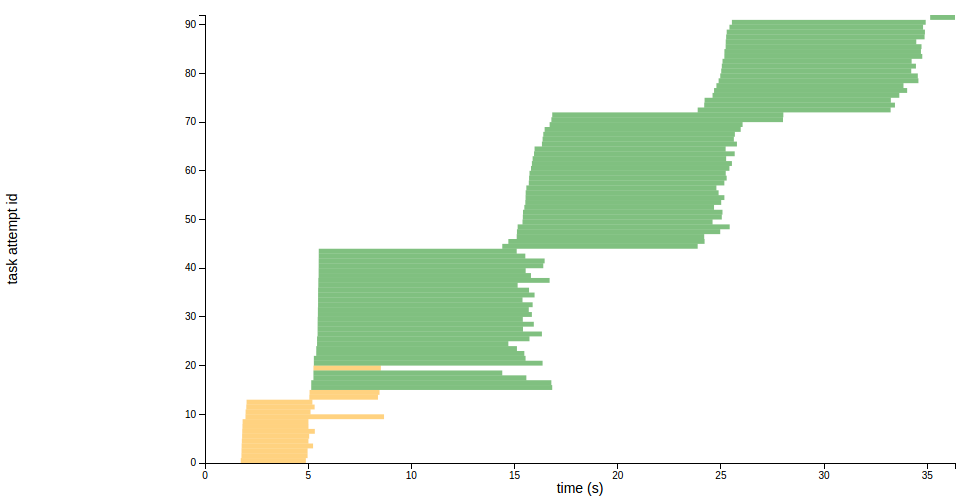
\includegraphics[width=0.4\textwidth]{fifo2.png}
  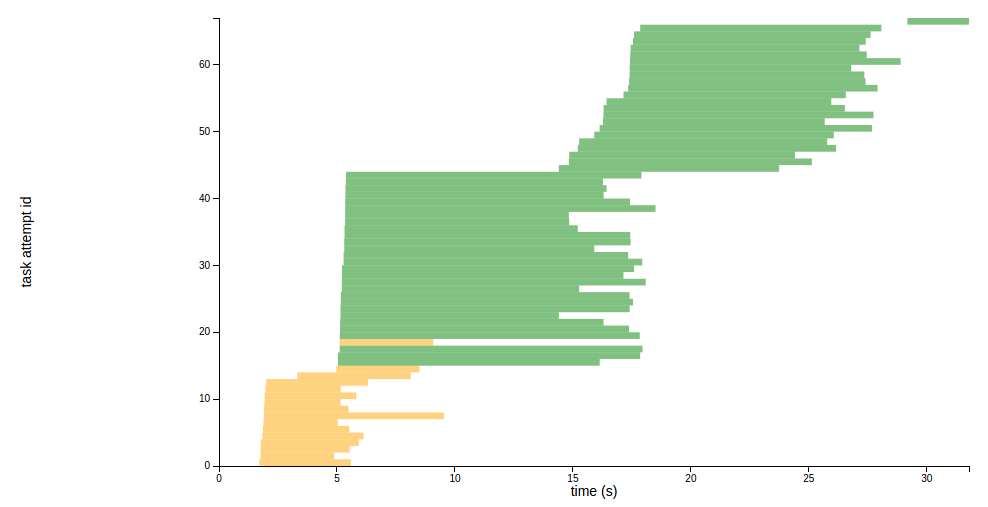
\includegraphics[width=0.4\textwidth]{fair2.png}
  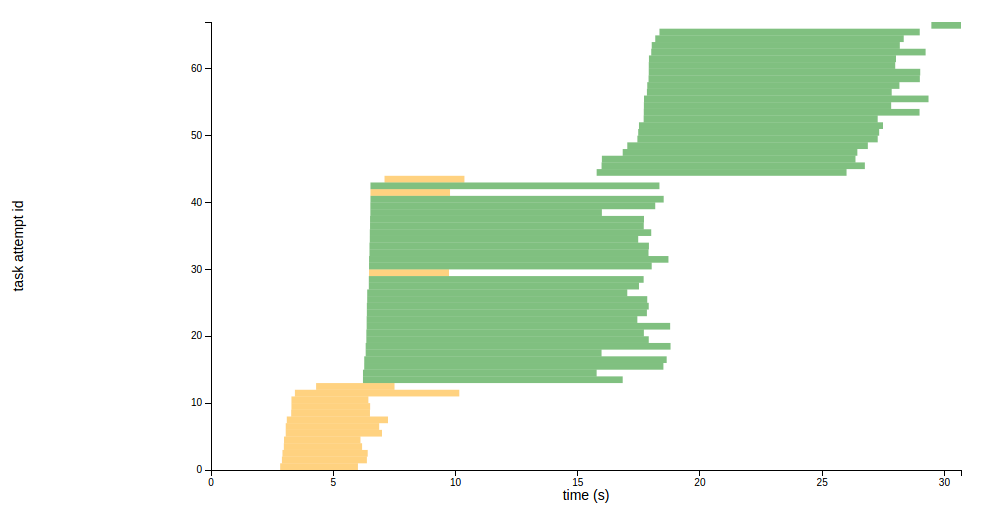
\includegraphics[width=0.4\textwidth]{fair_preemp2.png}
  \caption{Last sort applications with FIFO (left), Fair without preemption (right) and Fair with preemption (below)}
  \label{fair}
\end{figure}


\end{document}
